
\section{Evaluation}
\label{sec:evaluation}

For our evaluation, we implement PerfRanker based on Soot for static analysis and Java Agent for profiling the base version. 

%In this section, we first introduce the selection of subjects and code commits in subsection~\ref{subsec:subjects}, and introduce the evaluation setup and environment in Subsection~\ref{subsec:setup}. Then, we introduce the metrics for effectiveness measurement in Subsection~\ref{subsec:metrics}, and the evaluation results in Subsection~\ref{subsec:results}. (points-to analysis, call-graph building, control flow analysis, and data flow analysis for correlating collection variables and loops)  (dynamic call graph, iteration number of loops, and execution time of methods)
\subsection{Evaluation Subjects}
\label{subsec:subjects}

We apply PerfRanker on two popular open source projects: Xalan~\cite{xalan} and Apache Commons Math~\cite{commonMath}. Specifically, Xalan is an XSLT processor, and Apache Commons Math is a library for mathematical operations. We choose these two projects to cover both data formatting and mathematical computations, which are two representative time-consuming components in modern software. Xalan is equipped with a performance test suite of 64 test cases. Since Apache Commons Math is not equipped with a performance test suite, we leverage its unit test cases as performance test cases. 

\textbf{Version Selection.} For Apache Commons Math, we use its version on Jan 1, 2013 as its base version. For Xalan, since there are very few code commits after 2013, we use version 2.7.0 as its base version, as 2.7.0 is the first Xalan version compatible with Java 6 and higher. For both software projects, we collect all code commits from the base version until Mar 17, 2016, the time when we started collecting data for our work.  From all code commits, we remove those that do not change source files and those that do not involve semantic changes (e.g., renaming variables), as developers can easily determine that those commits will not affect software performance. Furthermore, we choose as our code-commit set the top 15 code commits whose changed code portions are covered by most test cases, where test prioritization is most needed. 

%For each selected code commit, we execute test cases on the commit for 5,000 times to determine performance regressions.

In Table~\ref{tab:subjects}, we present some statistics of the studied subjects and versions. The table shows that either project has more than 300K lines of code. Furthermore, there are hundreds of code commits and changed files between the base version and our selected code commits. In our evaluation, we do not update the base version, so the overhead of profiling the base version is low compared with the number of code commits under study.  More details about our evaluation subjects can be found on our project website~\cite{perfranker}.

\begin{table}
	\centering
	\caption{Evaluation Subjects}	
	
	
	\label{tab:subjects}
	\begin{tabular}{|l|r|r|} 
		\hline
		Subject  & Xalan  & Apache Commons Math  \\ 
		\hline
		Base Ver. & 2\_7\_0 & Jan 1st, 2013 \\ 
		\hline
		Size (LOC) of Base Ver. & 413,534   & 398,171  \\ 
		\hline		
		\# Commits Since Base Ver. & 354   & 1,321 \\ 
		\hline
		\# Changed Files  & 1,206  & 1,613 \\ 
		\hline
		Last Commit Date &Aug 11, 2015&Mar 17, 2016     \\ 
		\hline
%		Loop Exercise By Test & 364                         & 4151                             \\ \hline
	\end{tabular}
	\vspace{+1cm}
\end{table}





%We choose xalan version 2.7.0 as base version because version 2.6 is not compatible to jdk 1.6 to upper version. Benchmarking framework for XSLT, developed by Saxonica contains a set of test material, a set of test drivers for various XSLT processors, and tools for analyzing the test results.In the benchmark  we found 128 performance test case and only 64 of them run successfully with Xalan version 2.7.0. Similarly we chose 3900 test case for common math and studied the commits from github between  Dec 29, 2012 and Mar 17, 2016.

\subsection{Evaluation Setup}
\label{subsec:setup}


To determine performance regressions as the ground truth of performance changes for all test cases and code commits, we execute  the test cases for 5,000 times on the base version and each code commit under study. Furthermore, we execute the base version with our Java Agent to record the dynamic call graph and the execution time of each method, as well as the iteration number of each loop. To record average execution time of methods defined in the JDK library, we execute the Dacapo benchmark 9.12~\cite{dacapo} with profiling (we remove Xalan from the benchmark to avoid bias). All the executions are conducted on a Dell x630 PowerEdge Server with 32 cores and 256GB memory, and the server is used exclusively for our evaluation to avoid noises. 


%In Table~\ref{tab:profile}, we show top 5 frequently called JDK API methods and their average execution time in nano seconds. As described in Section~\ref{subsec:model}, this profile data is used in estimating the execution time of newly reached method bodies defined in JDK. 

%\begin{table}[] 
%	\small
%	\centering
%	\caption{Profiling Results}
%	\label{tab:profile}
%	\begin{tabular}{|l|r|r|} 
%		\hline
%		JDK api               & Average Time (ns)                      & Frequency               \\ \hline
%		java.util.Iterator:hasNext & 18	& 84,651,629  \\ \hline
%		java.util.Iterator:next	& 110	& 75,253,712  \\ \hline
%		java.util.List:get	& 22	& 38,302,721  \\ \hline
%		java.util.Map:get	& 100	& 21,632,743  \\ \hline
%		java.util.List:add	& 37	& 7,048,361  \\ \hline
%		... &            &   \\ \hline
%	\end{tabular}
%\end{table}


%We run the selected test sets on base version of each project and record context sensitive execution summaries of methods, loop counter and run time call graph. We can calculated average execution time of method and loop counter from all the profile data which is consider as global summary in our algorithm and local summary as per test case specific profile data. 
%We compared our approach to change aware random ranking which discussed in \ref{subsec:evaluation-result}. Prioritization technique metrics provide to testers the possibility to order their test cases so that test cases with large priority  are executed first and after test cases with less priority are executed in the regression testing process. APFD is commonly used to evaluate test case prioritization techniques to find functional fault. We adapt the metrics equation according to our needs in the formula \ref{eq:eq-apf}. In the formula p define as position in the ordering and IAPFD define as ideal APFD ranking.  The higher value of nAPFD signifies that highly impacted performance test case are in the top of ordering. 





\subsection{Evaluation Metrics}
\label{subsec:metrics}



To the best of our knowledge, our work is the first on prioritizing performance test cases for code commits, and we propose a set of metrics to evaluate the quality of different rankings. In our evaluation, we consider three ranking metrics: Average Percent of Fault-Detection on Performance (\textit{APFD-P}), normalized Discounted Cumulative Gain (\textit{nDCG}), and \textit{Top-N Percentile}. 

\textbf{APFD-P.} \textit{APFD}~\cite{AlexeyAPFD} is a commonly used metric for assessing a test sequence produced by test-case prioritization. If the test-suite size  is $N$, the total number of faults detected by the test suite is $T$, and the number of faults detected by the first $x$ test cases in the test sequence is $detected(x)$, then the \textit{APFD} of the test sequence can be defined in Formula~\ref{formula:apfd}:



\begin{equation}
APFD = \frac{\sum \limits_{x=1}^{N}\frac{detected(x)}{T}}{N} * 100\%
\label{formula:apfd}
\end{equation}


Unlike functional bugs where a test case either passes or fails, performance regressions are not binary but continuous. Performance downgrades of 20\% and 50\% are both regressions, with different severity. Therefore, instead of counting detected faults to attain the value of $detected(x)$, we replace the value of $detected(x)$ with the accumulated performance change. We define the \textit{performance change} of the $i^{th}$ test case in the test sequence (denoted as $change(i)$) in Formula~\ref{formula:impact} as below, in which $exe(i)$ is the execution time of the $i^{th}$ test case in the current version, and $exe(i_{base})$ is the execution time of the $i^{th}$ test case in the base version. 



 %Specifically, we define the performance change of a code commit on a test case as the relative change on execution time. 



\begin{equation}
change(i) = \frac{|exe(i) - exe(i_{base})|}{exe(i_{base})}
\label{formula:impact}
\end{equation}

Then, we define \textit{APFD-P} the same as  Formula~\ref{formula:apfd}, except that $detected(x)$ is defined as the accumulated performance change, as shown in Formula~\ref{formula:detect}, and $T$ is the sum of performance changes on all test cases. Actually, with such a definition, \textit{APFD-P} can be viewed as \textit{APFD} where all test cases reveal faults, and these faults are weighted by performance changes.

\begin{equation}
detected(x) = \sum_{i=1}^{x}change(i)
\label{formula:detect}
\end{equation}

As an illustrative example, consider 3 tests $t_1$, $t_2$, and $t_3$ with 10\%, 20\%, and 30\% performance downgrades, respectively. The best ranking is $t_3$, $t_2$, $t_1$; the total performance impact is $10\%+20\%+30\% = 60\%$; and the covered performance impact after each test is $30\%/60\% = 50\%$, $(30\%+20\%)/60\% = 83\%$, and $(30\%+20\%+10\%)/60\% = 100\%$. The P-APFD is thus (50\% + 83\% + 100\%)/3 = 78\%. 


%{\fontsize{7}{7}
%	\begin{multline}
%	\begin{gathered}
%	APFD_p =  \sum \limits_{i=1}^{p} impactRatio(p); \\
%	APFD = \sum \limits_{p=1}^{n} APFD_p \\
%	nAPFD = \frac{APFD}{IAPFD}
%	\label{eq:eq-apf}
%	\end{gathered}
%	\end{multline}
%}

\textbf{nDCG.} nDCG~\cite{NDCG} is a metric of ranking widely used in information retrieval. The basic idea is to calculate the relative score a given ranking with an ideal ranking, and the score of an arbitrary ranking is defined below, where $change(i)$ is defined in Formula~\ref{formula:impact}.

%and penalize each element that has high relevance score but is ranked lower in the given ranking with a value being logarithmic to the position difference. 

\begin{equation}
DCG (seq) = change(1) + \sum \limits_{i=2}^{N} \frac{ change(i)}{log_2(i)}
\label{formula:dcg}
\end{equation}


%In Formula~\ref{formula:dcg}, for a given sequence $seq$, we use the performance impact on the $i^{th}$ test case ($impact(i)$) as its relevance score, and $N$ to denote the length of $seq$, then the \textit{DCG} value of a given sequence $seq$ is defined in Formula~\ref{formula:dcg}. The \textit{nDCG} value of a given sequence $seq$ is its \textit{DCG} value normalized by the \textit{DCG} value of an ideal sequence, and is thus defined in Formula~\ref{formula:ndcg}, in which $ideal$ is the ideal ranking of the test cases (i.e., in descending order of performance changes).


%\begin{equation}
%nDCG (seq) = \frac{DCG(seq)}{DCG(ideal)}
%\label{formula:ndcg}
%\end{equation}


%The higher value of nDCG signifies that highly impacted performance test case are in the top of ordering.


\textbf{Top-N Percentile.} The \textit{APFD-P} and \textit{nDCG} defined earlier are adapted versions of widely used metrics, and can be used to compare different prioritization approaches. However, they are not sufficiently intuitive to help understand how much developers can benefit from an approach. Therefore, in our evaluation, we also measure how high percentage of top-ranked test cases in a test sequence need to be executed to cover the test cases with top $N$ performance impacts (we use 1 and 3 for $N$). For example, if the test cases with top 1, 2, and 3 performance impacts are ranked in the $2^{nd}$, $9^{th}$, and $5^{th}$ positions in a test sequence with length 100, then the top 1, 2, and 3 percentiles are 2\%, 9\%, and 9\%, respectively. 

\subsection{Baseline Approaches Under Comparison}

Although we are not aware of approaches specifically designed for prioritizing performance test cases in regression testing, it is possible to adapt existing approaches for performance test prioritization. In our evaluation, we compare our approach with three baseline approaches: Change-Aware Random, Change-Aware Coverage, and Change-Aware Loop Coverage.

Specifically, in all baseline approaches, we apply change-impact analysis to rule out the test cases that do not cover any revised methods. Since our performance-impact analysis includes basic change-impact analysis, for fair comparison, we apply this change-impact analysis in all baseline approaches. Note that we gathered coverage information from the base version, and we use the same technique as in our approach when selecting the code commits affecting most test cases in the three baseline approaches. 

After selecting the relevant test cases, the \textit{Change-Aware Random (CAR)} approach simply ranks the test cases in random order\footnote{To acquire more stable results, we use the average result of 100 random ordered test sequences as the result for CAR.}. The \textit{Change-Aware Coverage (CAC)} approach applies coverage-based test prioritization~\cite{Rother99:testprio} on the covered methods with the additional strategy~\cite{additionalTestPrior}, being a state-of-the-art approach in defect-oriented test prioritization. The basic idea is to first select the test case with the highest coverage, and iteratively select the test case that covers the most not-covered code portions as the next test case. In our evaluation, we use method coverage as the criterion, being consistent with the granularity of our performance model. The \textit{Change-Aware Loop Coverage (CALC)} approach is the same as CAC, except for using coverage of loops instead of methods as the criterion. 

\subsection{Quantitative Evaluation}
\label{subsec:results}
In our quantitative evaluation, we compare our approach and the three baseline approaches on all three metrics. 

\subsubsection{\textit{APFD-P} Metric}

%Our approach validated by real-world code changes and evaluate the tool on 354 commits of Xalan and 1321 commits of Apache common math.
%After filtering the result is shown in the figures. The filtered commits by our tool either only change non-source files or have insignificant changes on source files. Interestingly, filtering already reduces a significant number of commits not worth consideration for performance regression testing. We evaluated our result in three different metrics: APFD, DCG and Top Percentage aspect. In the case of APFD and DCG we compared our approach with change aware random approach. In change aware random, we generated 100 random ordering of test sets and calculated average nAPFD and nDCG. %APFD is computed after the prioritization only to measure the performance of the prioritization technique. 


Figures~\ref{fig:common-math-apfd} and~\ref{fig:xalan-apfd} show the comparison results between our approach and three baseline approaches on the \textit{APFD-P} metric. In the two figures and all the following figures, the X axis lists all the code commits studied chronologically, and the Y axis shows the \textit{APFD-P} value (or \textit{nDCG} value). We use different colors to represent different approaches consistently for all figures according to the legend in Figure~\ref{fig:common-math-apfd}. 

\begin{figure}
		\centering
		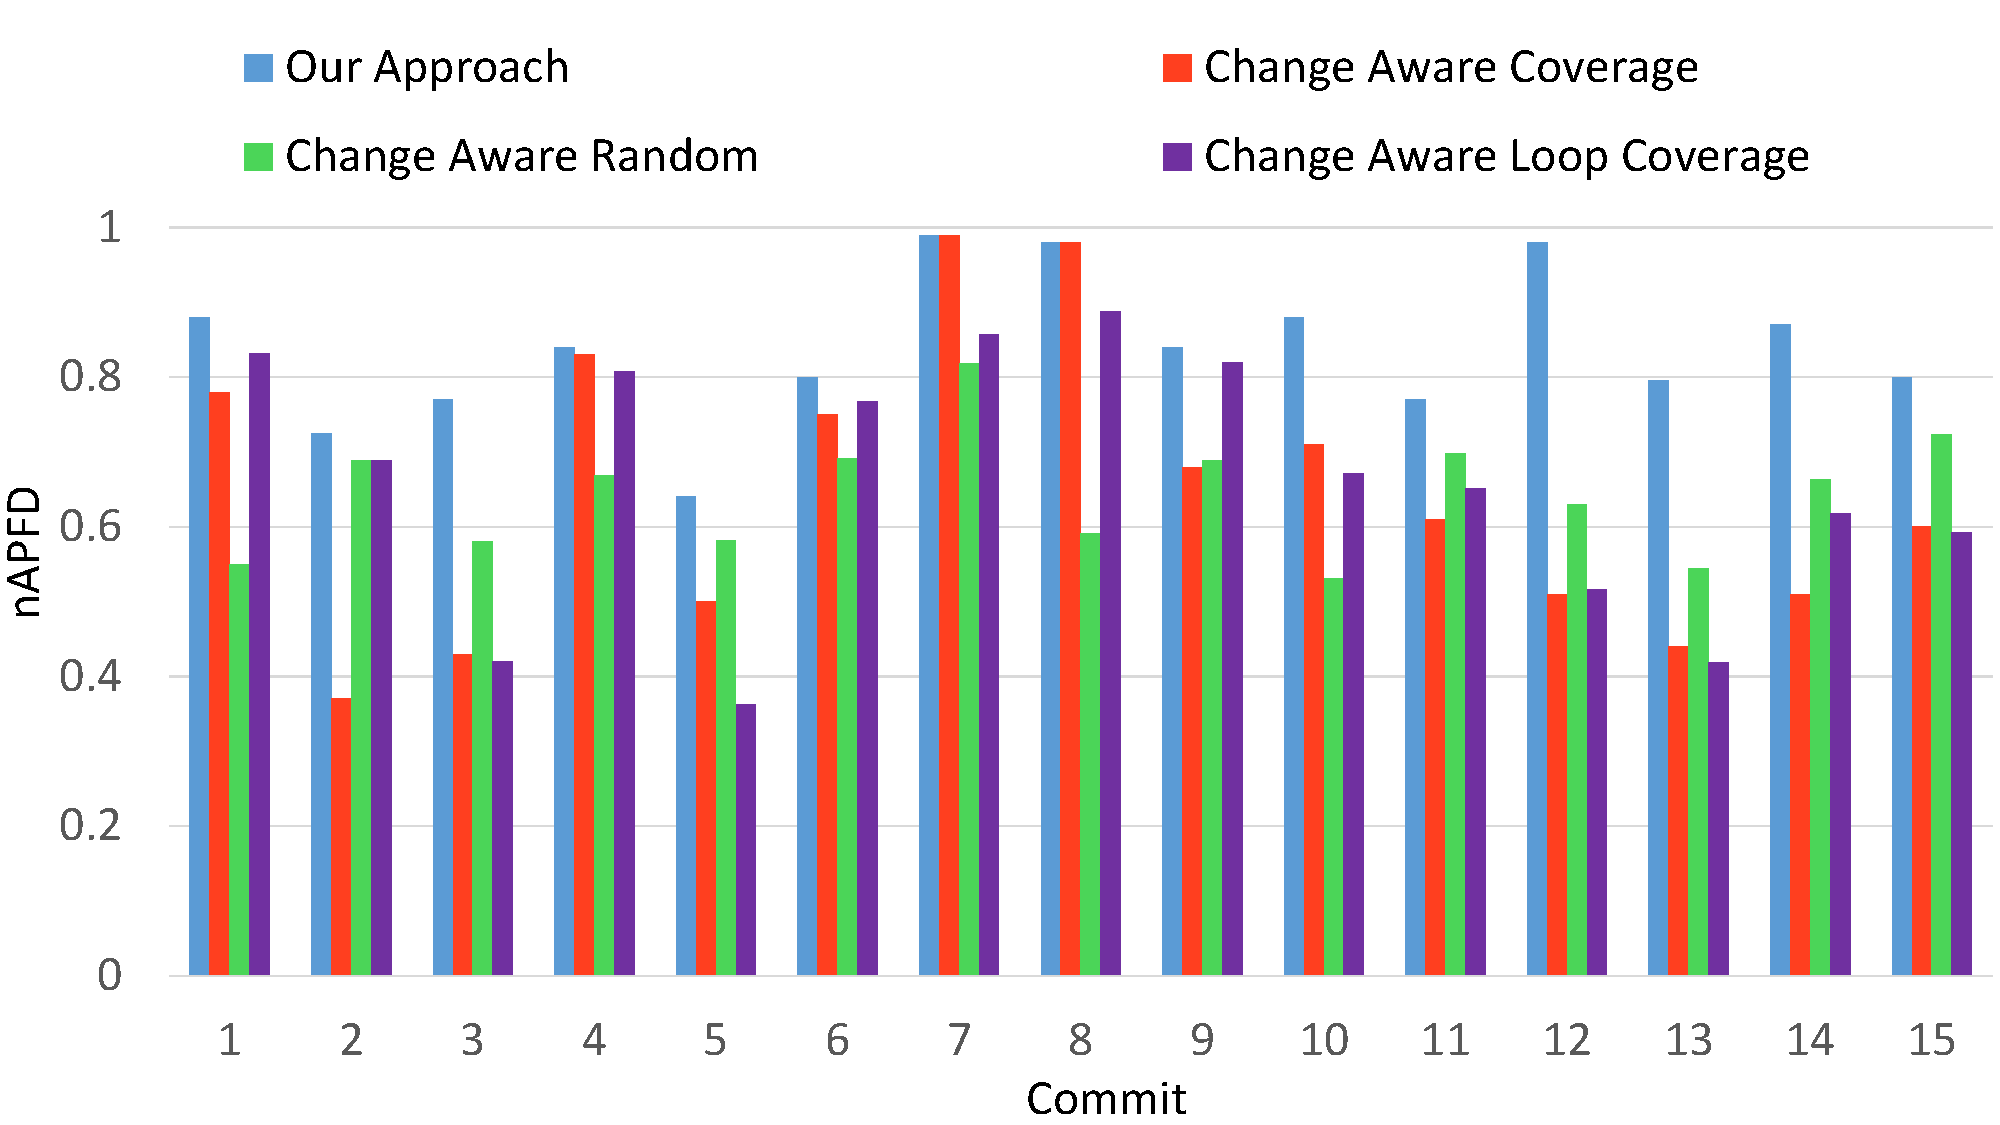
\includegraphics[width=4in, height=2.5in]{performance/images/common-math-apfd.pdf}
		
		\caption{\textit{APFD-P} Comparison on Apache Commons Math}	
		\label{fig:common-math-apfd}


\end{figure}

\begin{figure}
		\centering
		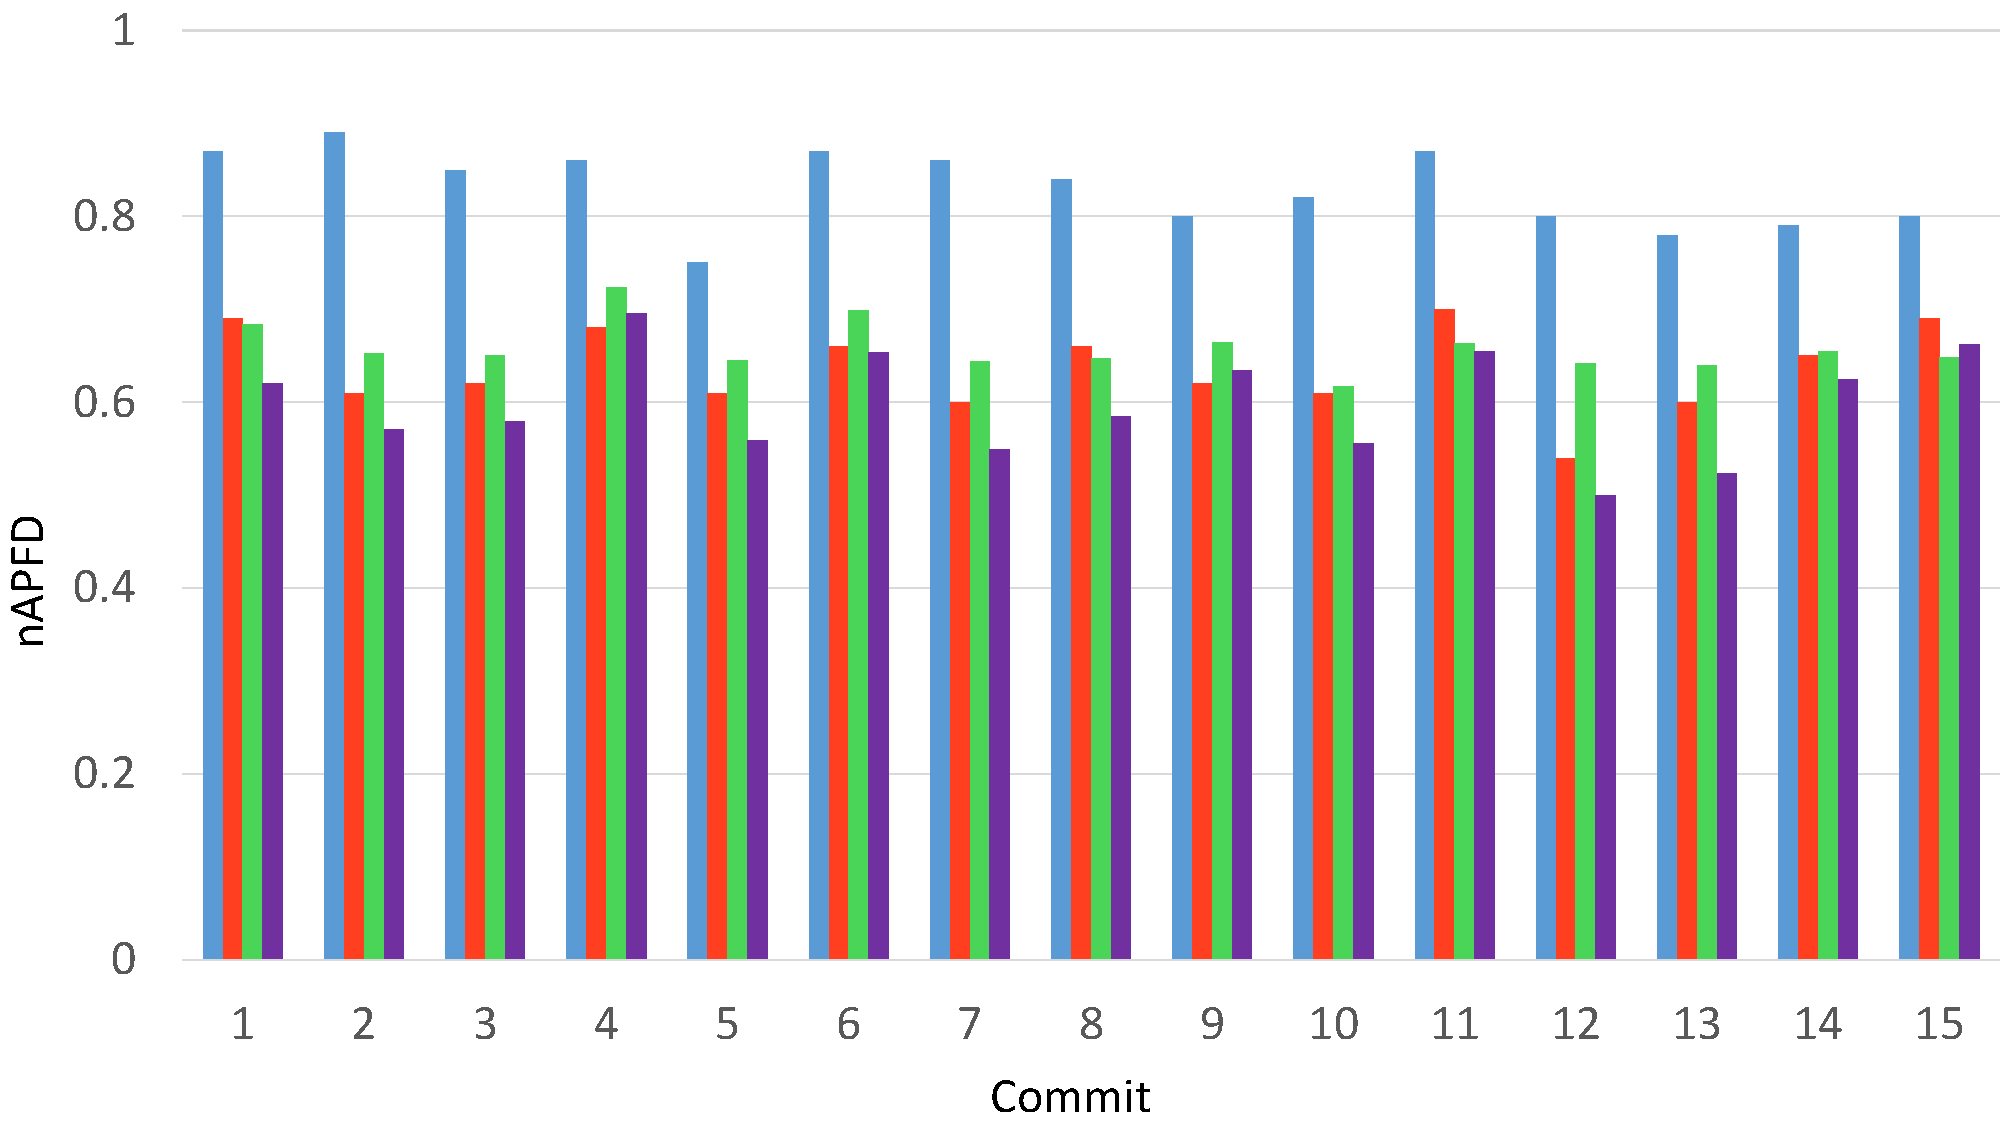
\includegraphics[width=4in, height=2.1in]{performance/images/xalan-apfd.pdf}
			
		\caption{\textit{APFD-P} Comparison on Xalan}
	
		\label{fig:xalan-apfd}
\end{figure}

%\begin{figure}
%		\centering
%		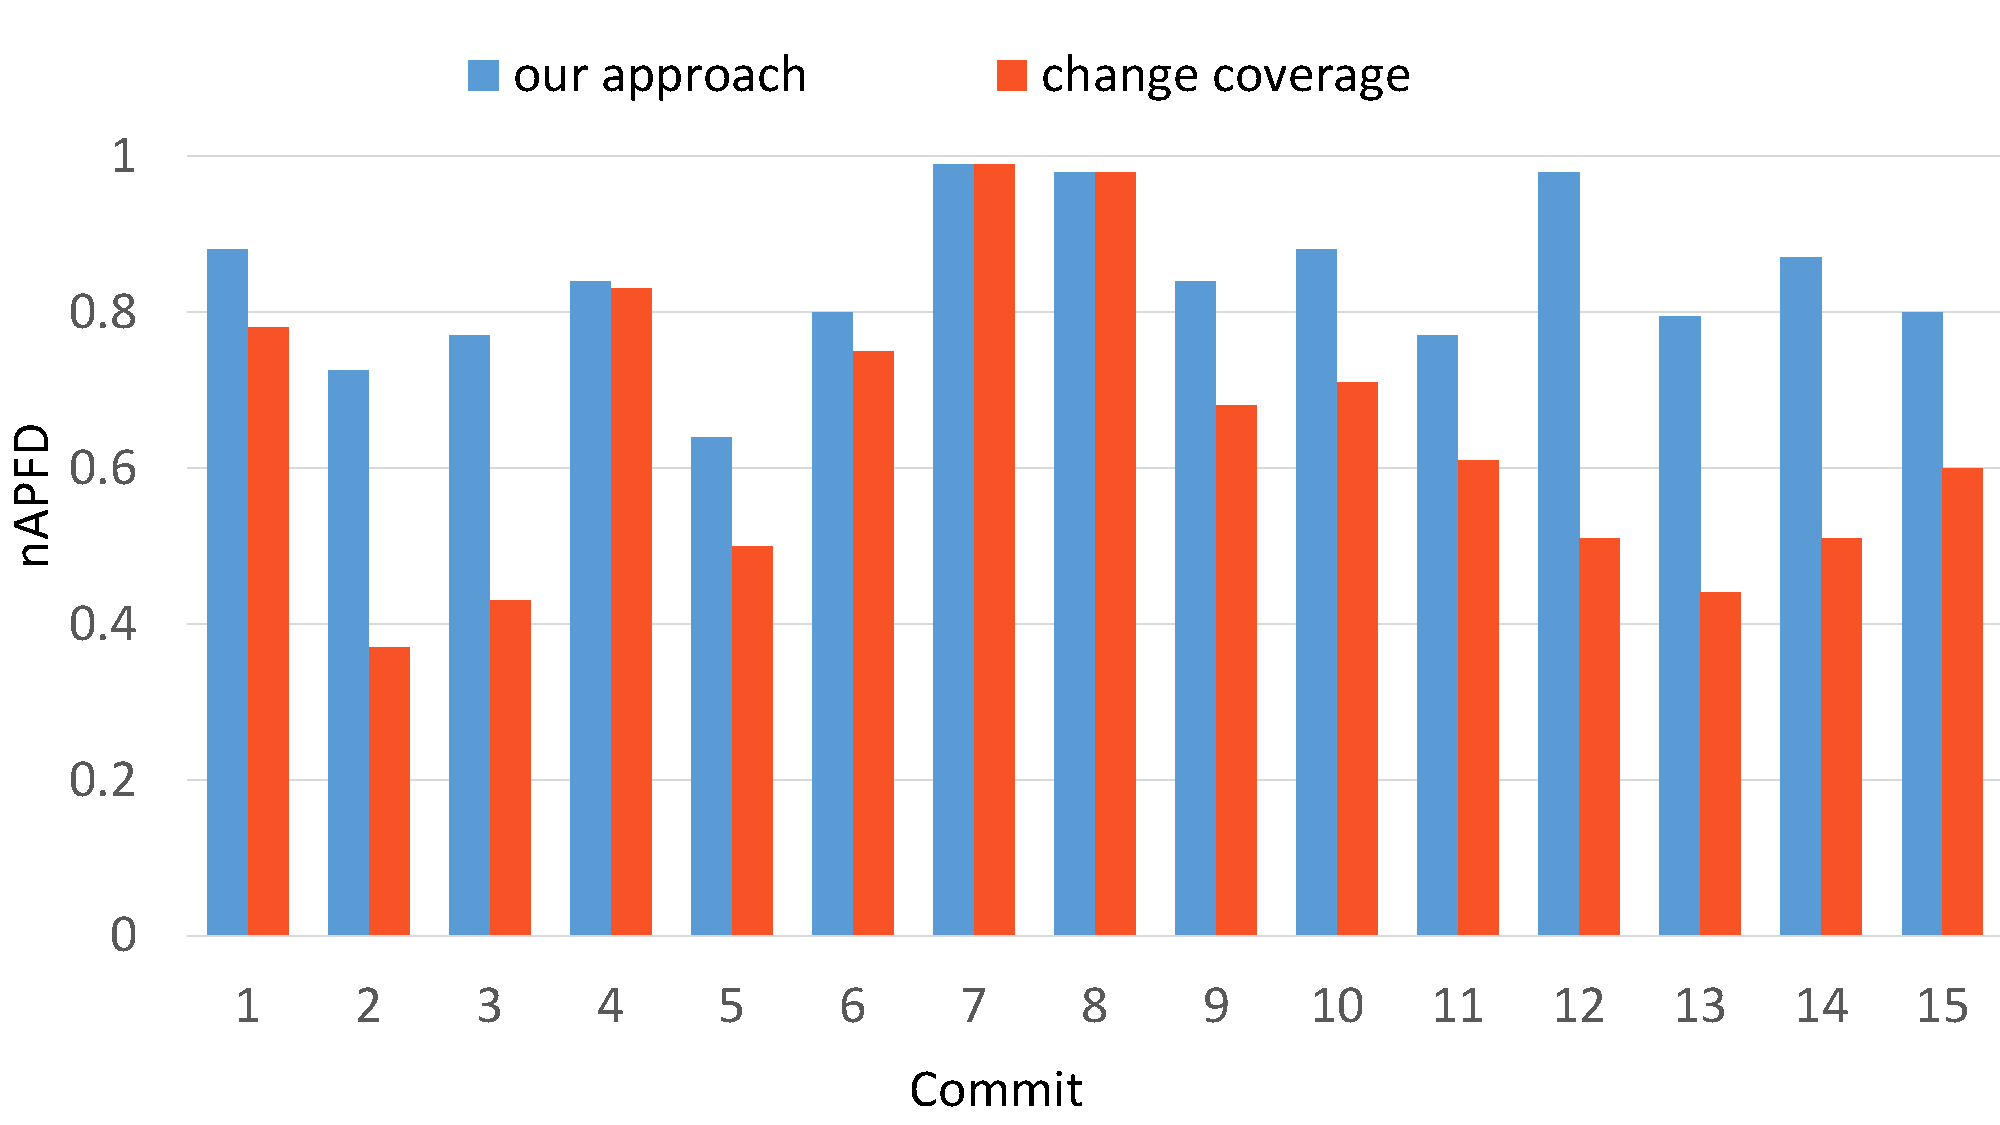
\includegraphics[width=\columnwidth]{images/common-math-coverage-apfd.pdf}
%		\caption{APFD-P Comparison with Change-Aware Coverage on Apache Commons Math}	
%		\label{fig:common-math-coverage-apfd}
%\end{figure}
%
%\begin{figure}
%		\centering
%		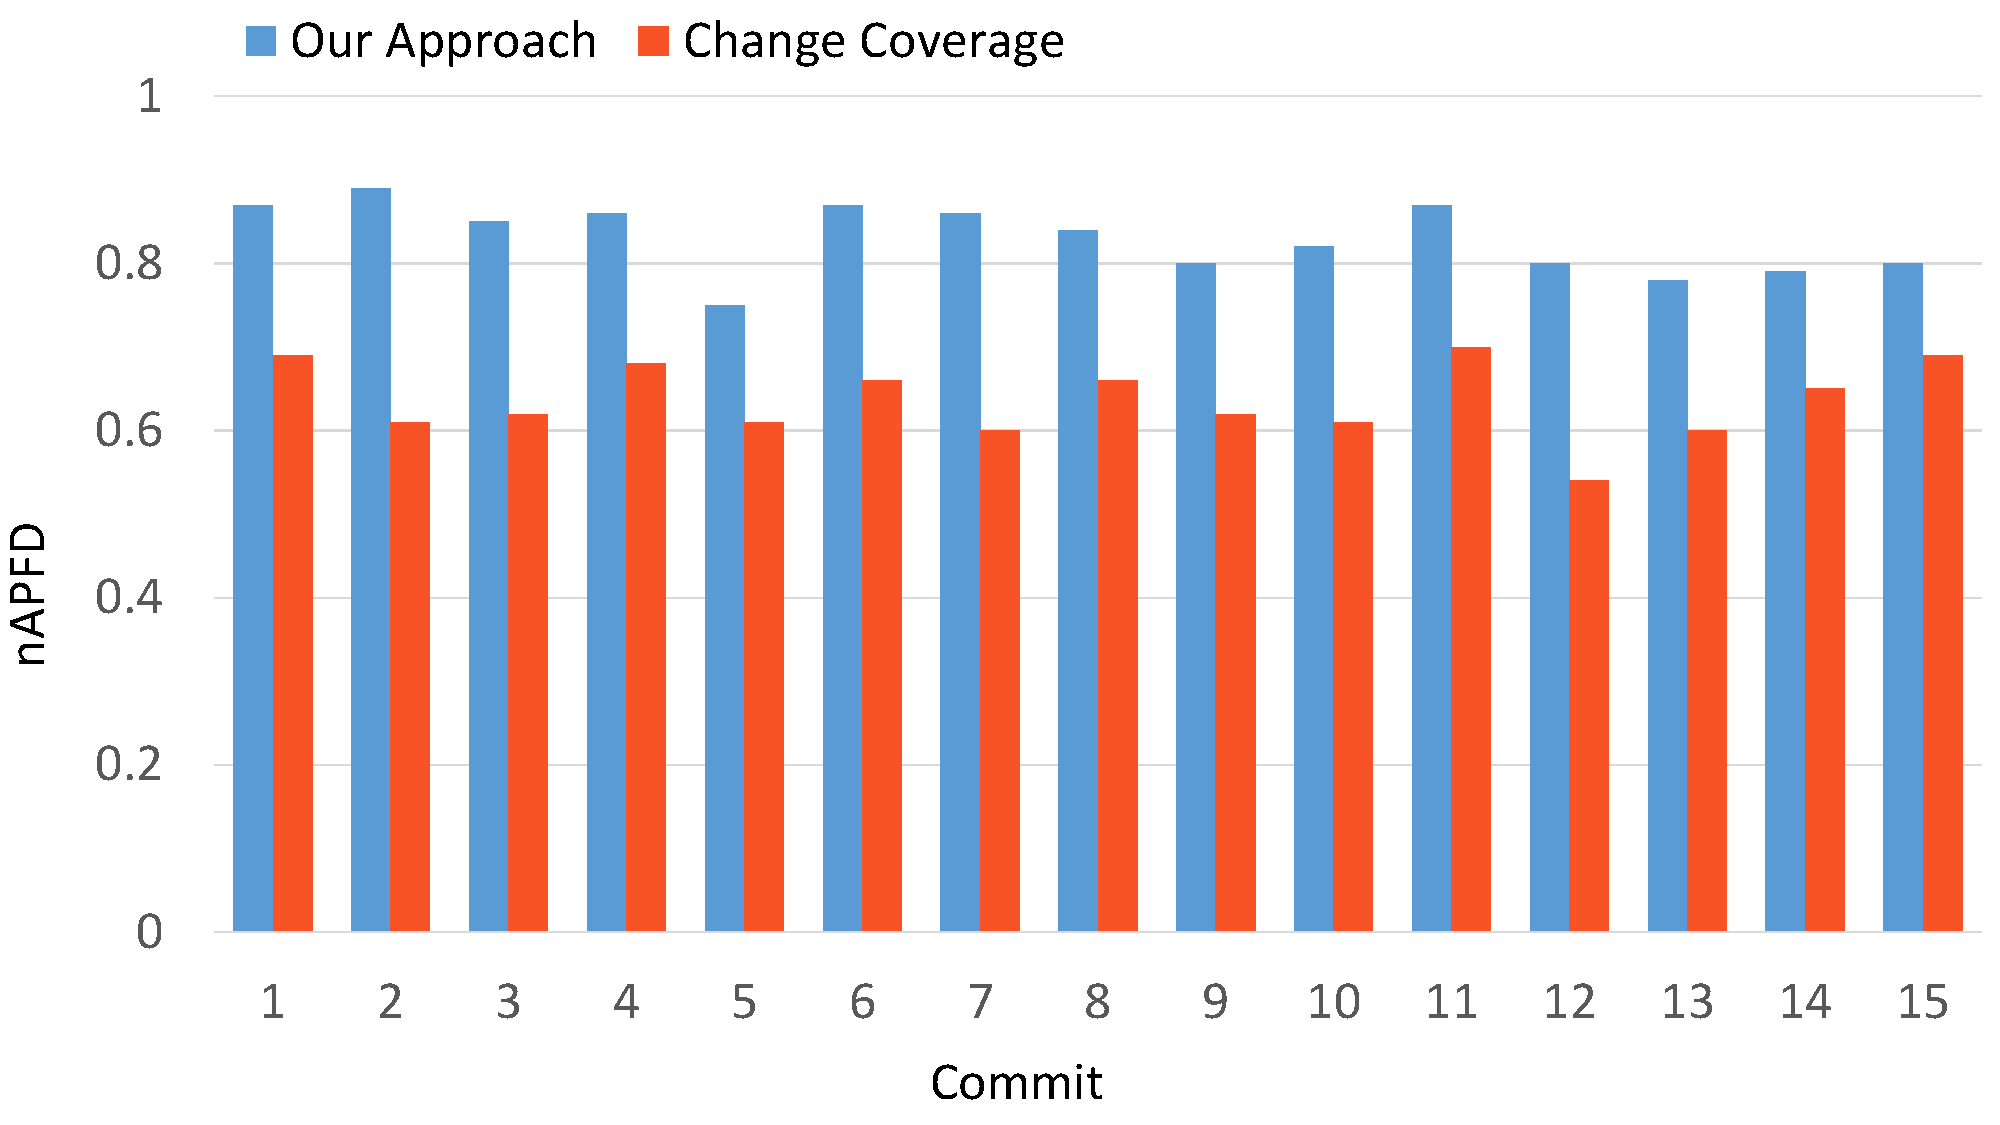
\includegraphics[width=\columnwidth]{images/xalan-coverage-apfd.pdf}
%		\caption{APFD-P Comparison with Change-Aware Random on Xalan}	
%		\label{fig:xalan-coverage-apfd}
%\end{figure}

Figures~\ref{fig:common-math-apfd} and~\ref{fig:xalan-apfd} show that our approach is able to achieve over 80\% \textit{APFD-P} value in most code commits affecting performance, and outperforms or rivals all baseline approaches in all code commits affecting performance from both subject projects. Specifically, for Apache Commons Math, our approach achieves an average \textit{APFD-P} value of 83.7\%, compared with 64.3\% by CAR, 64.6\% by CAC, and 66.1\% by CALC. For Xalan, our approach achieves an average \textit{APFD-P} value of 83.5\%, compared with 65.8\% by CAR, 63.6\% by CAC, and 59.8\% by CALC. Therefore, the improvement on the average \textit{APFD-P} is at least 17 percentage points, compared with baseline approaches on both projects. Furthermore, we do not observe significant effectiveness downgrade in the later versions, indicating that one base version can be used for a relatively long time.

%although we concede that the result may be due to the 

%Therefore, our approach is able to improve the APFD-P 


%In the figure \ref{fig:common-math-apfd}, we can see that overall nAPFD of our approach in Apache common math on the average 21.5\% greater than change aware random approach. In all the version our approach out perform random approach.





\subsubsection{\textit{nDCG} Metrics}

Similarly, Figures~\ref{fig:common-math-dcg} and~\ref{fig:xalan-dcg} show the comparison results between our approach and the three baseline approaches on the \textit{nDCG} metric. 

\begin{figure}
\centering
		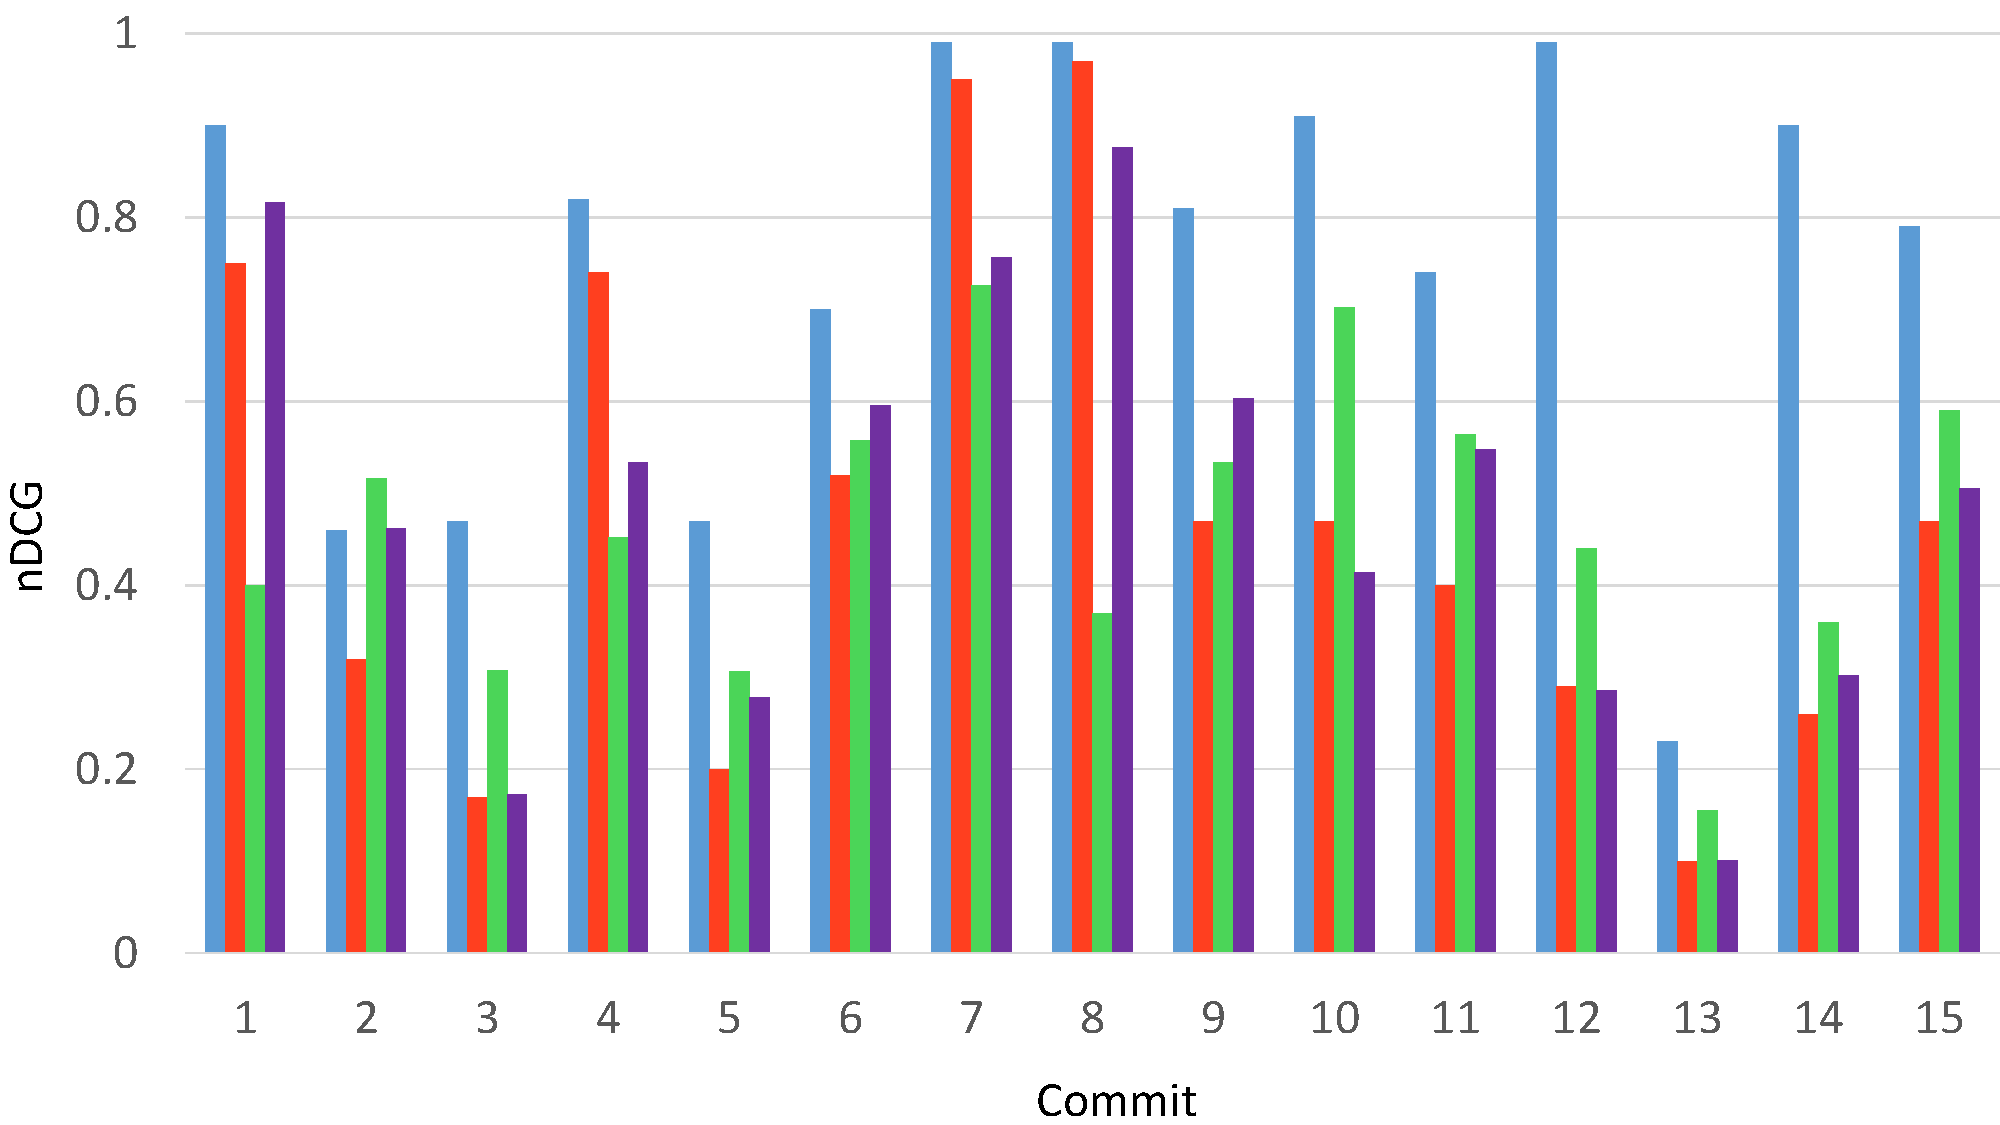
\includegraphics[width=4in, height=2.1in]{performance/images/common-math-dcg.pdf}
			
		\caption{\textit{nDCG} Comparison on Apache Commons Math}	
		\label{fig:common-math-dcg}
\end{figure}

\begin{figure}
\centering
		
		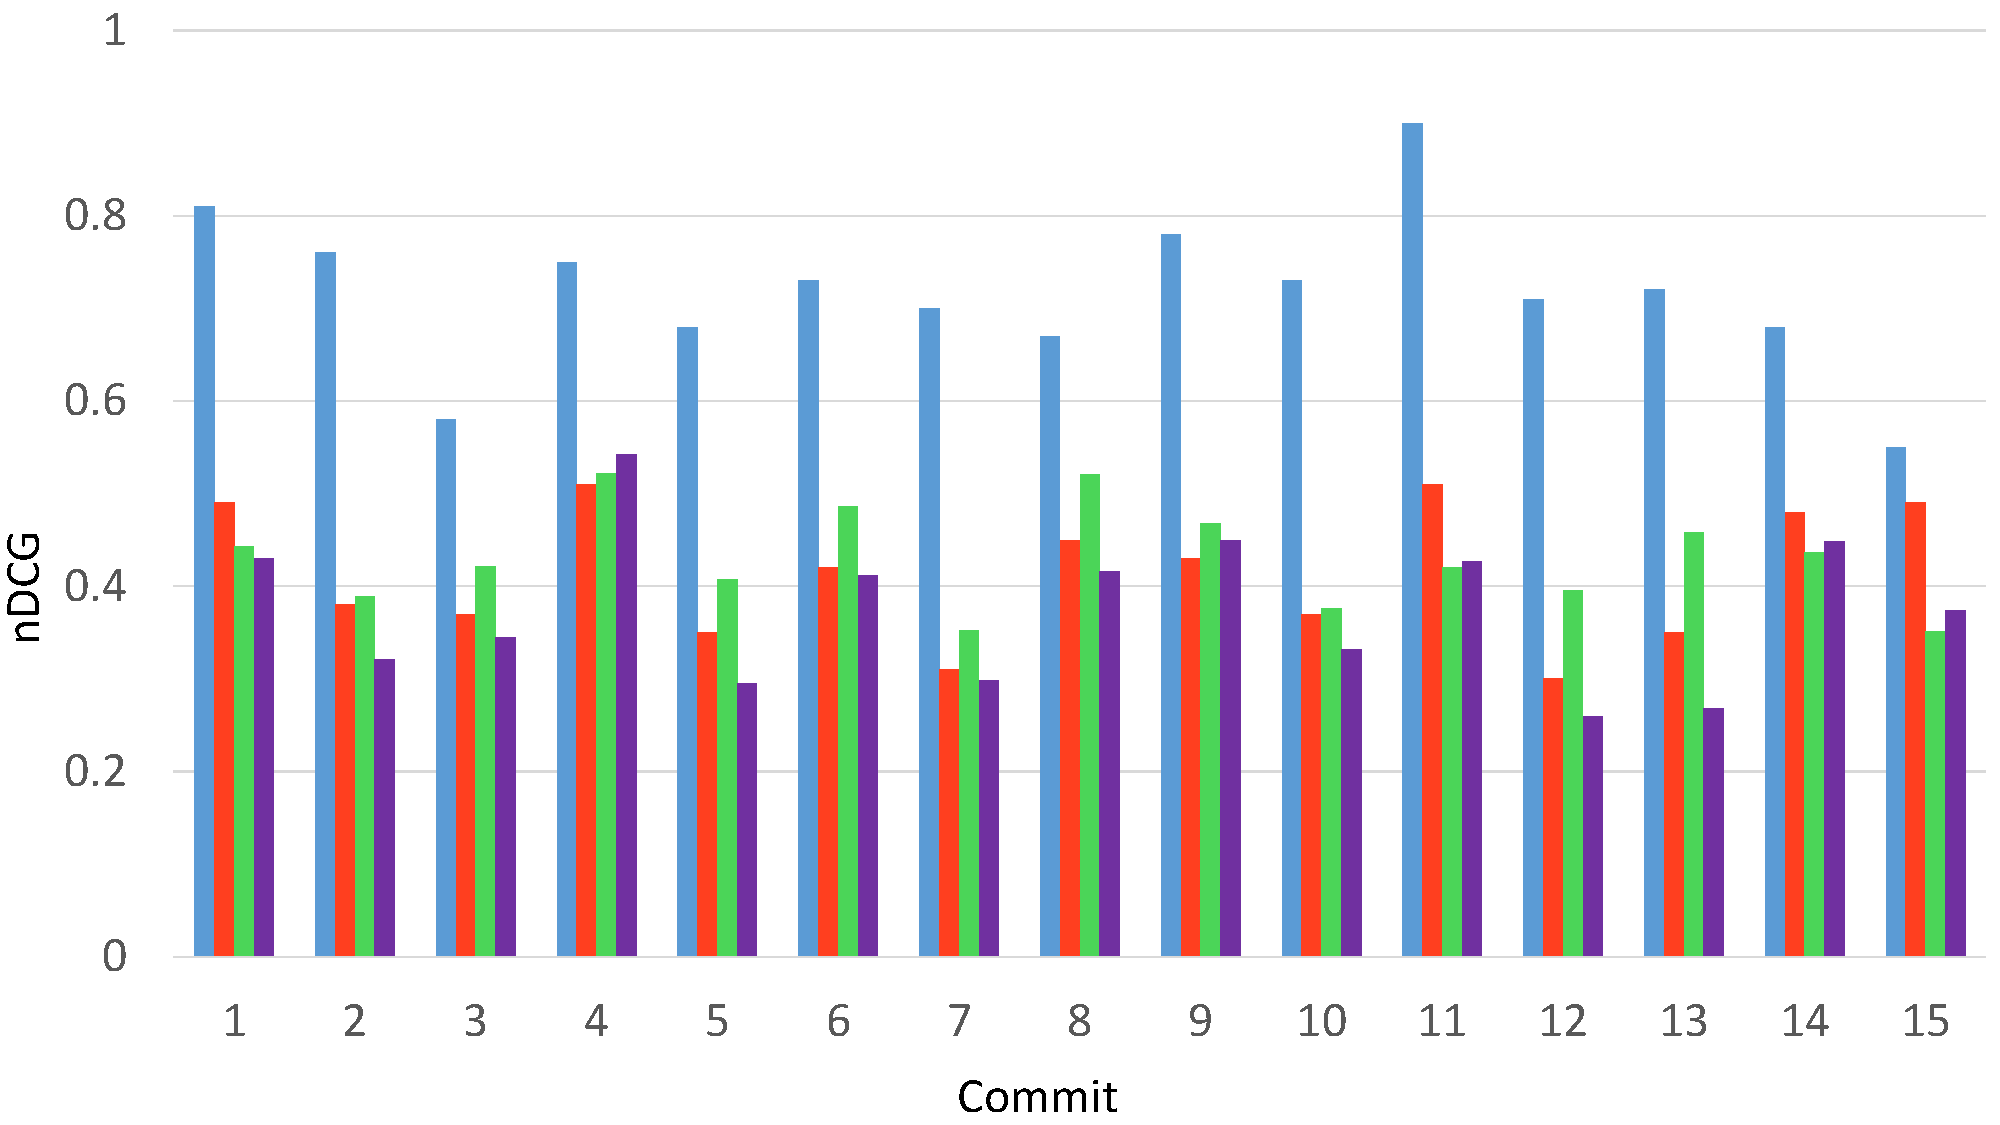
\includegraphics[width=4in, height=2.1in]{performance/images/xalan-dcg.pdf}
			
		\caption{\textit{nDCG} Comparison on Xalan}	
		\label{fig:xalan-dcg}
\end{figure}


%\begin{figure}
%		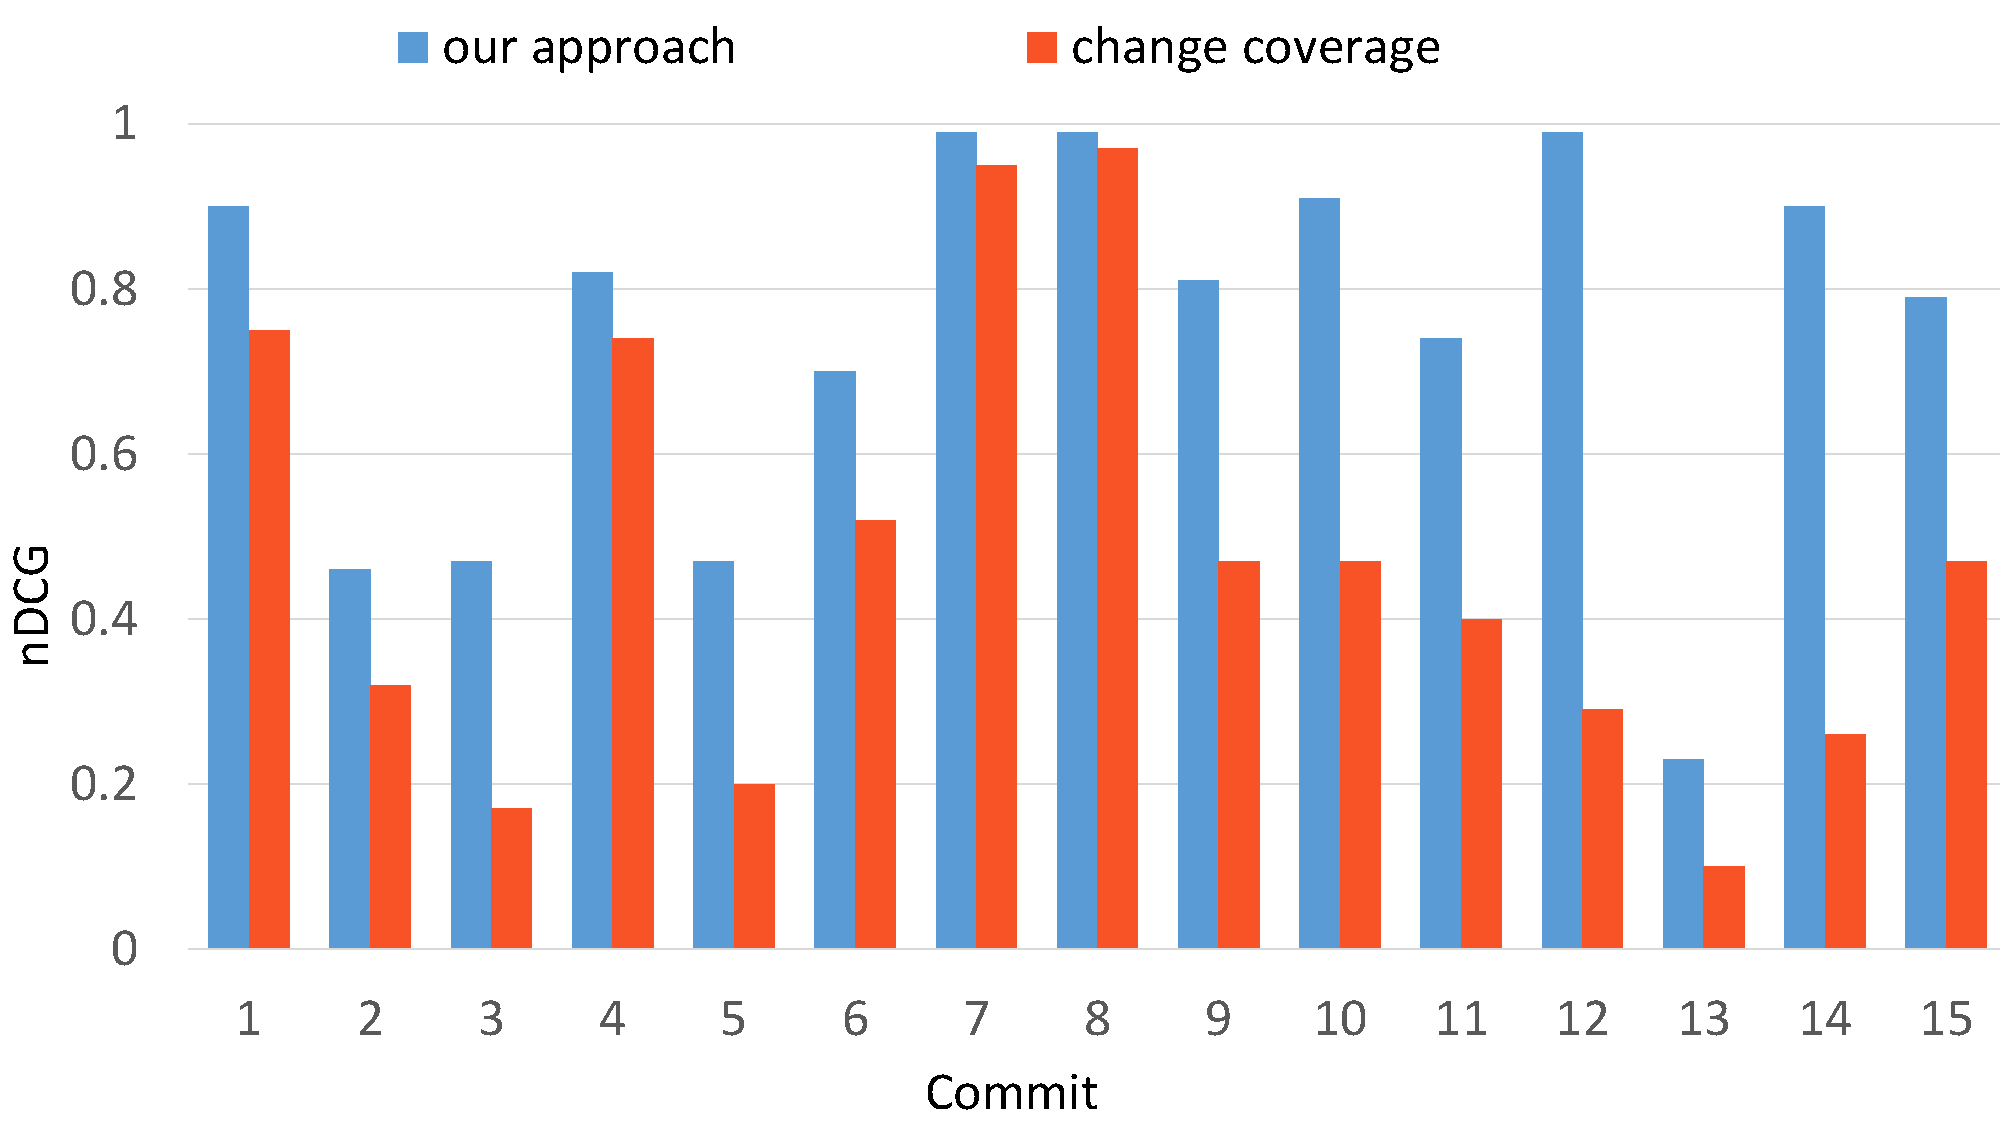
\includegraphics[width=\columnwidth]{images/common-math-coverage-dcg.pdf}
%		\caption{nDCG Comparison with Change-Aware Coverage on Apache Commons Math}	
%		\label{fig:common-math-coverage-dcg}
%\end{figure}
%
%\begin{figure}
%		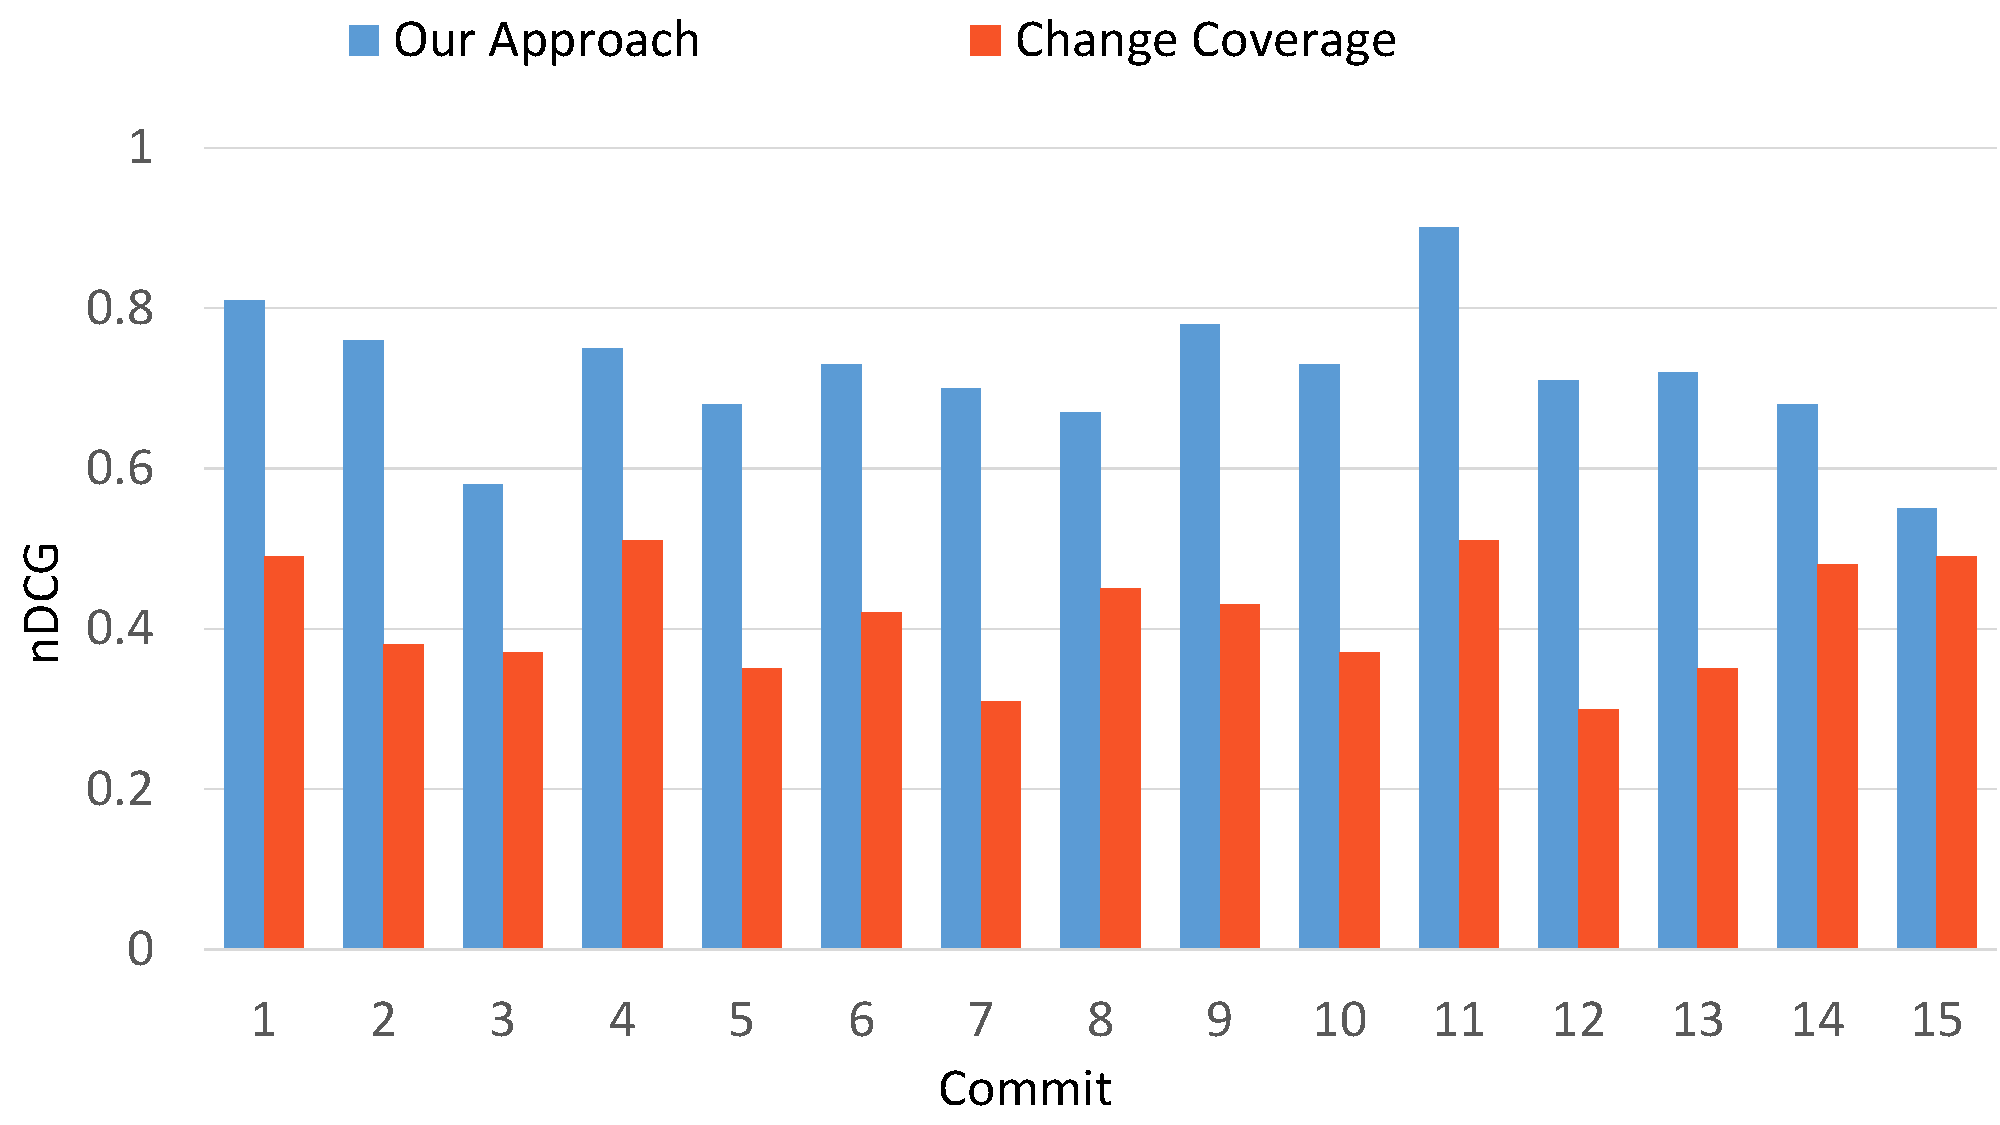
\includegraphics[width=\columnwidth]{images/xalan-coverage-dcg.pdf}
%		\caption{nDCG Comparison with Change-Aware Coverage on Xalan}	
%		\label{fig:xalan-coverage-dcg}
%\end{figure}

The figures show that our approach outperforms or rivals baseline approaches on \textit{nDCG} in almost all code commits from both subject projects. Specifically, for Apache Commons Math, our approach achieves an average \textit{nDCG} value of 74.5\%, compared with 47.2\% by CAR, 46.5\% by CAC, and 48.4\% by CALC. For Xalan, our approach achieves an average \textit{nDCG} value of 71.7\%, compared with 43.0\% by CAR, 41.4\% by CAC, and 37.4\% by CALC. Therefore, the improvement on the average \textit{nDCG} is over 26 percentage points on both projects. We also observe that there is one code commit from Xalan, in which our approach performs slightly worse than CAR on \textit{nDCG}. In Section~\ref{sec:qualitative}, we further discuss the details of this code commit in Listing~\ref{list:example-n1}.

Finally, we observe that compared with \textit{APFD-P}, the \textit{nDCG} values are generally lower and vary more significantly from code commit to code commit. The reason is that an \textit{nDCG} value is more sensitive to the rank of test cases with the highest performance impacts. For example, consider a test sequence with 100 test cases and only 1 test case has performance impact, and the performance impact value is 100\%. When this test case is ranked top, both \textit{APFD-P} and \textit{nDCG} are 1.0. However, if this test case is ranked $25^{th}$ in the sequence, the \textit{APFD-P} value is still as high as 75\%, but the \textit{nDCG} value becomes $1/log_2(25)$, which is less than 25\%. This result is reasonable because in information retrieval (where \textit{nDCG} was first  proposed), ranking the most relevant result at the $25^{th}$ position is very bad, but in test prioritization (where \textit{APFD} was first proposed), ranking the test case at the $25^{th}$ position is not so bad, because only 25\% test cases need to be executed to execute the test case. Therefore, which of \textit{APFD-P} and \textit{nDCG} is a better metric may depend on whether developers are interested in only a few most severely affected test cases, or a larger number of test cases whose performance is affected. 

%find that overall nDCG is higher comparison to nAPFD due to reason of penalising top impacted test case which are lower in the order. In some version improvement is much higher comparative to  


%The proposition of high nDCG is that highly relevant result appearing at the top. In the figure \ref{fig:common-math-dcg}, we can see that overall nDCG of our approach in Apache common math on the average 29.29\% greater than change aware random approach. 



%some other version for several reason is discussed above. Similarly, in the figure \ref{fig:xalan-dcg}, we can see that overall nDCG of our approach in Xalan on the average 27.21\% greater than change aware random approach.  \\
 


%We further compare our approach with change coverage approach. In figure \ref{fig:common-math-coverage-apfd}  and \ref{fig:xalan-coverage-apfd} shows the comparison of our approach with change coverage approach on  metric APFD. Our approach in common math on the average APFD score 0.85 whereas change coverage  average APFD score 0.68 (17\% greater). Similary, Our approach in xalan on the average APFD score 0.83 whereas change coverage  average APFD score 0.63 (19\% greater).In figure \ref{fig:common-math-coverage-dcg}  and \ref{fig:xalan-coverage-dcg} shows the comparison of our approach with change coverage approach on  metric DCG. Our approach in common math on the average DCG score 0.77 whereas change coverage  average DCG score 0.53 (24\% greater). Similary, Our approach in xalan on the average DCG score 0.71 whereas change coverage  average DCG score 0.41 (30\% greater).\\

\subsubsection{Top-N Percentile}

While \textit{APFD-P} and \textit{nDCG} are normalized quantitative metrics for our problem, they are not sufficiently intuitive for understanding the direct benefit of our approach on developers. Therefore, we further measure how many test cases developers need to consider if they want to cover the top 3 most affected test cases. Tables~\ref{tab:math} and~\ref{tab:xalan} show the results. Columns 1 and 2 present the code commit number and the total number of test cases affected by the code commit, respectively. Columns 3-6 and 7-10 present the top proportion of ranked test cases required to cover top 1 and 3 most-performance-affected test cases\footnote{The results for top 2 show similar trends and are available on the project website~\cite{perfranker}}. 

%In each column group, the first column presents our result, and the remaining columns present the results of CAC, CALC, and CAR, respectively. 

%In each cell, the number in the bracket shows the percentage of test cases need to be considered. 



\begin{table}
\scriptsize
	\centering
	\caption{Top-N Percentile of Apache Commons Math}
	\label{tab:math}	
	
	\begin{tabular}{r|r||r|r|r|r||r|r|r|r}
	\hline
C &T & \multicolumn{4}{c||}{Top 1} & \multicolumn{4}{c}{Top 3} 
\\  \cline{3-10}
\#  & \#   & Our & CAC & CALC & CAR &  Our & CAC & CALC & CAR\\\hline
	1 & 55 & 2\% & 3\%& \textbf{1\%} & 49\% & \textbf{6\%} & 43 & 27\%& 74\%\\
	2 & 60     & 40\%& 61\%& \textbf{38\%} & 49\% & \textbf{51\%} & 61\% & 93\% & 74\%\\
	3 & 152     & \textbf{2\%} & 84\%& 79\%& 49\%  & \textbf{28\%} & 88\% & 88\% & 74\% \\
	4 & 97      & \textbf{3\%} & 18\%& 87\% &  49\%  & \textbf{5\%} & 18\% & 87\% & 74\% \\
	5 & 130    & \textbf{4\%} & 29\% & 43\% & 49\% & \textbf{4\%} & 96\% & 97\% & 74\%  \\
	6 & 15     & \textbf{13\%} & 40\%& 33\%&46\% & 66\% & \textbf{40\%} & 100\% &  73\% \\
	7 & 18      & \textbf{5\%} & \textbf{5\%} & 88\% & 47\% & \textbf{15\%} & 40\% & 88\% & 74\%\\
	8 & 10     & \textbf{10\%} & \textbf{10\%} & 40\% &45\%  & \textbf{60\%} & \textbf{60\%} & 70\%& 70\%\\
	9 & 12     & \textbf{8\%} & 66\%&75\% & 45\% & \textbf{50\%} &66\% & 75\%& 72\%\\
	10 & 12      & \textbf{8\%} & 50\% & 83\% & 45\% & 83\% & \textbf{50\%} & 100\% & 72\% \\
	11 & 36      & \textbf{5\%} & 94\%& 38\% & 48\% & 66\% & 94\%& \textbf{58\%} & 74\%\\
	12 & 13     & \textbf{7\%} & 76\% & 38\%& 45\% & 76\% & 84\%& 100\%& \textbf{72\%} \\
	
	13 & 711    & \textbf{7\%} & 81\%& 84\% & 49\% & \textbf{7\%} & 81\%& 84\%& 74\% \\
	14 & 39      & \textbf{2\%} & 84\%& 25\%& 48\% & \textbf{12\%} & 84\% & 79\% & 74\% \\
	15 & 34      & \textbf{11\%} & 52\% & 17\% & 48\% & \textbf{26\%} & 58\%& \textbf{26\%} & 74\%\\ \hline
	Avg      &   & \textbf{8\%} & 50\% & 51\% & 48\%  & \textbf{37\%} & 65\% & 78\% & 73\% \\  \hline
	\end{tabular}
\end{table} 

\begin{table}
\centering 
\caption{Top-N Percentile of Xalan}
	
\label{tab:xalan}
\scriptsize
\begin{tabular}{r|r||r|r|r|r||r|r|r|r}
\hline
C &T & \multicolumn{4}{c||}{Top 1} & \multicolumn{4}{c}{Top 3} 
\\  \cline{3-10}
\#  & \#   & Our & CAC  & CALC & CAR&  Our  & CAC  & CALC & CAR\\\hline
1 & 63     & 20\%& 46\% & \textbf{14\%} & 49\% & \textbf{36\%} & 60\% & 50\% & 74\% \\
2 & 63   & \textbf{17\%} & 85\% & 22\% & 49\%& \textbf{17\%} & 85\%& 80\%&74\% \\
3 & 63      & \textbf{7\%} & 85\% & 50\% & 49\%  & \textbf{38\%} & 85\% & 66\% & 74\% \\
4 & 63   &  20\%& 80\% & \textbf{7\%} & 49\% & \textbf{20\%} & 85\% & 73\% & 74\% \\
5 & 63   & \textbf{6\%} & 85\% &  100\% & 49\% & \textbf{53\%}  & 85\% & 100\% & 74\%\\
6 & 63      & \textbf{11\%} & 63\% & 31\% & 49\% & \textbf{26\%} & 76\% & 77\% & 74\% \\
7 & 63   & \textbf{11\%} & 46\% &  12\% & 49\% & \textbf{15\%} & 85\% & 93\% & 74\% \\
8 & 63    & \textbf{9\%}  & 35\% & 36\% & 49\% & \textbf{20\%} & 82\% & 95\% & 74\% \\
9 & 58      & \textbf{3\%} & 96\% &  5\% & 49\% & \textbf{25\%} & 96\% & 98\% & 74\% \\
10 & 63   & 30\% & 47\% & \textbf{17\%} & 49\% & \textbf{31\%} & 85\% & 84\% & 74\% \\
11 & 63   & \textbf{1\%} & 31\% & 12\% & 49\% &  \textbf{7\%}  & 62\% & 74\% & 74\% \\
12 & 63     & \textbf{23\%} & 85\% & 88\% & 49\% & \textbf{34\%} & 90\% & 88\% & 74\%\\
13 & 63     & \textbf{12\%} & 46\%& 82\% & 49\%  & \textbf{53\%}  & 65\%& 82\% &74\% \\
14 & 58    & 34\% & 34\% & \textbf{8\%} & 49\% & 43\% & \textbf{37\%}  & 72\% & 74\% \\ 
15 & 63     & 36\% & \textbf{4\%} & 12\% & 49\% & \textbf{36\%} & 79\%& 61\% & 74\% \\ \hline
Avg        & & \textbf{16\%} & 57\%  & 34\% & 49\%& \textbf{30\%} & 77\%  & 79\% & 74\% \\		\hline
\end{tabular}
\end{table}

%For example, change version-3 touches 13 test case and actual impact score of top test case 1st,2nd and 3rd are 0.75, 0.07 and 0.06 respectively. Our approach ranked them with impact score 7.57,2.36 and 2.35 where overall nAPFD score of approach is 0.98 compared to change aware random score 0.63 that is 35\% improvement.


%Performance regression testing cost reduction is highly desirable. For example, running few top impacted test case can save a lot of testing time. Keep that goal in mind, we evaluated our result and We consider only those changes that touches more than three test case in the table \ref{tab:math} and \ref{tab:xalan}. 

Tables~\ref{tab:math} and~\ref{tab:xalan} show that on average our approach is able to cover Top 1 and 3 most-performance-affected test cases within top 8\%, 21\%, and 37\% of ranked test cases in Apache Commons Math, and 16\%, 22\%, and 30\% of test cases in Xalan. The improvements over the baselines approaches are at least 33\%, 37\%, and 28\%. Furthermore, on top 1 coverage, our approach outperforms or rivals the best baseline approach on 13 code commits from Apache Commons Math, and 10 code commits from Xalan. On top 3 coverage, our approach achieves the highest percentage on 11 code commits from Apache Commons Math, and 14 code commits from Xalan. 

%Also, our approach generates better result for Top 1 for code commits affecting fewer test cases, but better result for Top 3 for code commits affecting more test cases. The major reason is that, for code commit affecting fewer test cases, maybe only 1 or 2 test cases are affected with high performance impact. So the 3rd most affected test case may be not very different from other test cases. Actually, one drawback of using Top N coverage as metrics is that, it does not taking into account the actual performance impact, which is considered in $APFD-P$ and $nDCG$.


%consistently better than the two baseline approaches on most code commits, and 


\subsubsection{Overhead and Performance}
In test prioritization, it is important to make sure that the time spent on prioritization is much smaller than the execution time of performance test cases. To confirm indeed that is the case, we record the overhead and execution time of our analysis. Our profiling of the base version has a 1.92 times overhead on Apache Commons Math, and 5.18 times overhead on Xalan. The static analysis per test case takes 29.90 seconds on Apache Commons Maths, and 34.35 seconds on Xalan. Finally, for Apache Commons Math, the average, minimal, and maximal time for analyzing a code commit are 45.35 seconds, 4.23 seconds, and 262.30 seconds, respectively, while for Xalan, the average, minimal, and maximal time for analyzing a code commit are 9 seconds, 3.36 seconds, and 21.80 seconds, respectively. In contrast, it takes averagely 52 (3) minutes to execute test suite of Apache Commons Math (Xalan) for 173 (47) times to achieve an expectation of equal to or less than 10\% execution-time variance.


%we can see that, top1 contains on the average within 8\% in common math and 16\% in xalan. That means more than 85\% test cases can be eliminated. Similarly top2 and top3 contain on the average within  21\% and 37\% respectively in common math and   22\% and 30\% respectively in common xalan. So on the average our approach eliminate 70\% test case to select top 3 impacted test case.


%These table show the result of Top1, Top2 and Top3 impacted test case position in the ranking order and contain within percentage result of apache common math and xalan. For example, first row in the table \ref{tab:math} represents that the changes in version-1 impacted test case 1st, 2nd and 3rd position in the ranked list is 11th,1st and 2nd respectively and top 3 impacted test case contain within 17\% in the ranked list. The changes in version-9 touches 55 test cases and their relative ordering perfectly match the actual ordering of top 3. The main reason is that relative impact difference between the test case distinguishable which means that 1st relative impact 3 to 5 times compared to 2nd and 3rd in this case. But the change on version-13 touches 711 test cases and the impact on test case are very similar and little difference in their relative order which is top1's relative impact score 1.05 to 1.13 times compared to 2nd and 3rd. Within 0.54 score interval contains 653 test case. So we can say that a good separation margin in performance impact among the order test case provide better ranking order. Though their position in the ranking above 50, top 3 contains within 7\%. 


%There is another commit version where our approach perform better than random but it is below 25\% compared to ideal. It is interesting that top 3 contain within 7\% in the ranked list which means it can eliminate 93\% test case. The reason of this issue is explained in later paragraph under Top percentage result evaluation. 



%\subsubsection{Summary of Findings}
%To sum up, our quantitative analysis has the following major findings. 

%\begin{itemize}
%	\item Our technique outperforms both 
%	\item 
%\end{itemize}


\subsection{Successful and Challenging Examples}
\label{sec:qualitative}
%In all the version our approach out perform random approach except one version which touches 60 test case and interestingly top 3 contain within 51\%. Though our approach is below random in this case, it can eliminate 60\% test case to select top impacted test case. The overall ranking does not perform well in this change because of the reason that conditional return or throws statement  added in the top of method body is shown in the listing\ref{fig:example-2}. As a result some of test case skip the whole execution of method which spend time inside loop in the method body in earlier version. 

In this section, with representative examples of code commits, we explain why our approach performs well on some code commits but not so well on some others. 

%Due to space limit, for each code commit, we present only the relevant changes instead of the whole commit. More details about our code commit examples can be found on our project website~\cite{perfranker}.

\textbf{Successful Example 1.} Listing~\ref{list:example-p1} shows the simplified code change of code commit hash d074054... of Xalan. On this code commit, our approach is able to improve the \textit{APFD-P} and \textit{nDCG} values by at least 13.53 and 31.22, respectively, compared with the three baseline approaches. In this example, several statements are added inside a loop. Our approach can accurately estimate the performance change because (1) Line 2 in the code is an existing loop and from the profile database for the base version we can find out exactly how many times it is executed, and (2) the added method invocations are combinations of existing method invocations whose execution time is already recorded for the base version. \\

%Combining the information in our performance model, we can precisely predict the performance impact of the change for each test case.


{\fontsize{10}{10}
\begin{lstlisting}[columns=flexible,language=Java,caption=Change Inside a Loop, label={list:example-p1}]
  int nAttrs = m_avts.size();
  for (int i = (nAttrs - 1); i >= 0; i--){
    ...
+   AVT avt = (AVT) m_avts.get(i);
+   avt.fixupVariables(vnames, cstate.getGlobalsSize());
    ...
  } 
\end{lstlisting}
}


\textbf{Successful Example 2.} Listing~\ref{list:example-p2} shows the simplified code change of code commit hash 64ec535... of Xalan. On this code commit, our approach is able to improve the \textit{APFD-P} and \textit{nDCG} values by at least 17.14 and 24.33, respectively, compared with the baseline approaches. In this example, the loop at Line 4 depends on the collection variable \CodeIn{m\_prefixMappings} at Line 1 whose size can be inferred from the recorded number of iterations of existing loops. In this case, our approach can accurately estimate the iteration count of this new loop and estimate the overall performance impact based on the estimated iteration count.\\

{\fontsize{10}{10}
	\begin{lstlisting}[columns=flexible,language=Java,caption=A Newly Added Loop Correlating to an Existing Collection, label={list:example-p2}]
	+ int nDecls = m_prefixMappings.size();
	+      
	+ for (int i = 0; i < nDecls; i += 2){
	+   prefix = (String) m_prefixMappings.elementAt(i);
	+   ...
	+ }     
	\end{lstlisting}
}

%Our approach can easily identity hot path and changes that lie in the hot path from our performance model which is constructed on the call graph. Beside these any intra procedure change that related to loop can estimate impact cost except few cases. But we believe that actual improvement is more than this score because running the regression with top impacted test case is enough for exposing performance problem and the probability of selecting top impacted test case 7\% in random. 

%Collection are generally propagated through function parameter and field variable. In Listing~\ref{list:example-p3}, at line 1 introduce new array list and at line 6 this list is updated under a existing loop. We can easily estimate the length of new array list. New method introduce that is not shown here that iterate of over the new list, our technique can predict the iteration of that loop. 

%{\fontsize{7}{7}
%\begin{lstlisting}[language=Java,caption=Collection Propagation, label={list:example-5}]
%+ Collections.sort(limits);

%+ for (int i = 0; i < limits.size(); i += 2) {
%  +list.add(new Arc(limits.get(i), limits.get(i + 1)));
%+}
%\end{lstlisting}
%}

%{\fontsize{7}{7}
%	\begin{lstlisting}[language=Java,caption=Correlation New and Existing Collection, label={list:example-p3}]
%	+ List processedDefs = new ArrayList();
%	
%	for (int i = 0; i < nAttrs; i++){
%	+
%	
%	+ processedDefs.add(attrDef);
%	+
%	
%	}
%	\end{lstlisting}
%}

%\textbf{Positive Example 3.} The simplified code change of code commit of Apache common math is presented in Listing~\ref{list:example-p3}. On this code commit, our approach is able to enhance $APFD-P$ and $nDCG$ by at least 34.12, and 48.35, compared with 3 baseline approaches but it is not presented in $APFD-P$ and $nDCG$ graph because the number of test cases affected by the change are less than 10. In Listing~\ref{list:example-p3}, at Lines 3-5, elements from the collection variable \CodeIn{limits} are added to another collection variable \CodeIn{list}. In this case, our collection propagation technique is able to link the two collection variables, and propagate the impact to the loops depending on variable \CodeIn{list}. It should be noted that, the iteration number of the loop is actually half of the size of \CodeIn{limits}. In our approach, for simplicity, we ignore different operations on the index variables and simply deem the loop-iteration numbers to be the same as the size of collections it depends on. Since test prioritization does not require exact prediction of performance impact, we found our approach to be still effective with such approximations (e.g., in this example). 
%
%{\fontsize{7}{7}
%\begin{lstlisting}[language=Java,caption=Collection Propagation, label={list:example-p3}]
%+final List<Arc> list = new ArrayList<Arc>();
%+ Collections.sort(limits);
% + for (int i = 0; i < limits.size(); i += 2) {
%  +list.add(new Arc(limits.get(i), limits.get(i + 1)));
%+}
%\end{lstlisting}
%}
%
%Although our approach is almost consistently better than the two baseline approaches and the improvement is significant, we still want to investigate the cases where our approach does not perform well (e.g., the one case where our approach performs worse than Change-aware Random, and the cases where the improvement is not significant). 

\textbf{Challenging Example 1.} Listing~\ref{list:example-n1} shows the simplified code change of code commit hash 90e428d... of Apache Commons Math. On this code commit, with respect to the \textit{nDCG} metric, our approach performs better than the CAC baseline approach but slightly worse than the CAR baseline approach. In the example, at Line 2, an invocation to method \CodeIn{checkParameters()} is added, and the method may throw an exception. In this example, the execution time of \CodeIn{checkParameters()} can be easily estimated with our performance model. However, if the exception is thrown, the rest of the method will not be executed. Although we are able to estimate the execution time of the method's remaining part, it is impossible to estimate the probability of throwing the exception, as \CodeIn{checkParameters()} is a newly added method without any profile information. In such cases, if the probability of throwing the exception is higher in some test cases, the reduction of execution time due to the exception will be the dominating factor and result in inaccuracy in our prioritization.\\ 


{\fontsize{10}{10}
\begin{lstlisting}[columns=flexible,language=Java,caption=Return or Throw Exception at Beginning, label={list:example-n1}]
  protected PointVectorValuePair doOptimize(){
+   checkParameters();
    ...	
  }
+ private void checkParameters() {
+   ...
+   throw new MathUnsupportedOperationException;
+ }
\end{lstlisting}
}


\textbf{Challenging Example 2.} There are also cases where developers added a loop that is not relevant to any existing collection variables. As one of such examples, Listing~\ref{list:example-n2} shows the simplified code change of code commit hash a51119c... of Apache Commons Math. On this code commit, the improvement of our approach over the best result of the three baseline approaches is only 0.8 for \textit{APFD-P} and 6.0 for \textit{nDCG}. 
%
In the example, Line 2 introduces a new loop that does not correlate to any existing collection or array. In such a case, our approach cannot determine the iteration count of this loop and the depth of recursion at Line 8. To still provide prioritization results, our approach uses the average iteration counts of all known loops to estimate the iteration count of this new loop and always estimates the recursion depth to be 1. However, our prioritization result becomes less precise due to such coarse approximation.\\

{\fontsize{10}{10}
\begin{lstlisting}[columns=flexible,language=Java,caption= New Loop with No Correlation, label={list:example-n2}]
  public long nextLong(final long lower, final long upper){
+   while (true) {
      ...
+     if (r >= lower && r <= upper) {
+       return r;
+     }              
+   }
+   return lower + nextLong(getRan(), max);  
 }
\end{lstlisting}

}


%In some version improvement is much higher comparative to  some other version for several reason. For example,in the listing\ref{list:example-2} conditional return or throws statement  added in the top of method body introduce complex logic which is hard to determine which test case execute the full body of the method. As a result introduce imprecise impact cost. Another reason is that a new method is added with a loop in the listing \ref{list:example-1} and 


\subsection{Threats to Validity}

Major threats to internal validity are potential faults in the implementation of our approach and baseline  approaches, potential errors in computing evaluation results of various metrics, and the various factors affecting the recorded execution time for the test cases. To reduce such threats, we carefully implement and inspect all the programs, and execute the test cases for 5,000 times to reduce random noises in execution time. Major threats to external validity are that our evaluation results may be specific to the code commits and subjects studied. To reduce the threats, we evaluate our approach on both data processing/formatting software and mathematical computing software, and both a unit test suite and a performance test suite. 

%Also, we use an objective standard to select the code commits where test prioritization is most useful. To further reduce the threat, we plan to evaluate our approach on more subject projects and more code commits. 

